\section{Results} 

\begin{figure}[h]
 \centering
 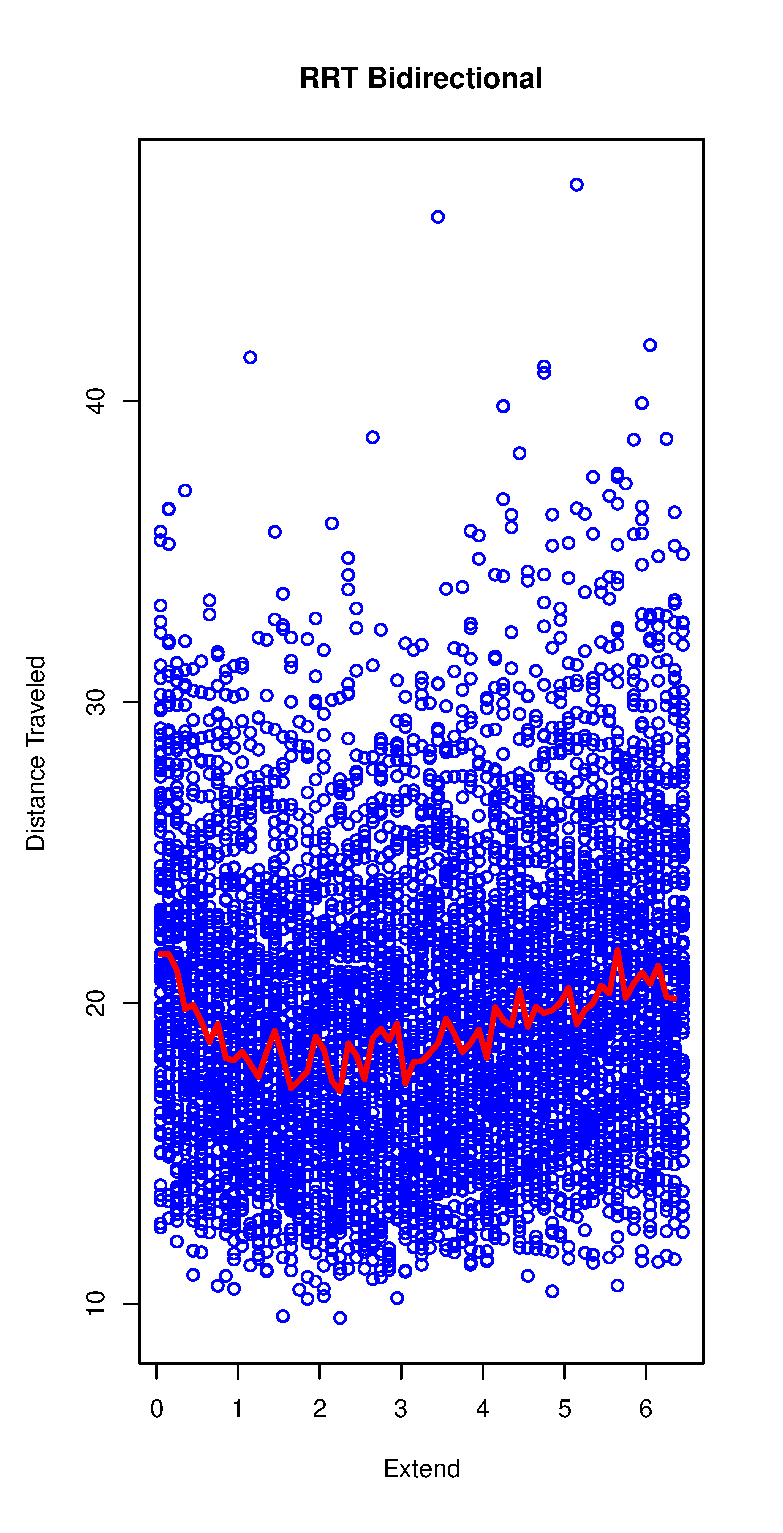
\includegraphics[width=\figsize]{graphics/bidirectional_correlation}
 \caption{\(d_J\) of the bidirectional RRT planner (blue) with median highlighted (red).}
 \label{fig:bidir_correlated}
\end{figure}

\begin{figure}[h]
 \centering
 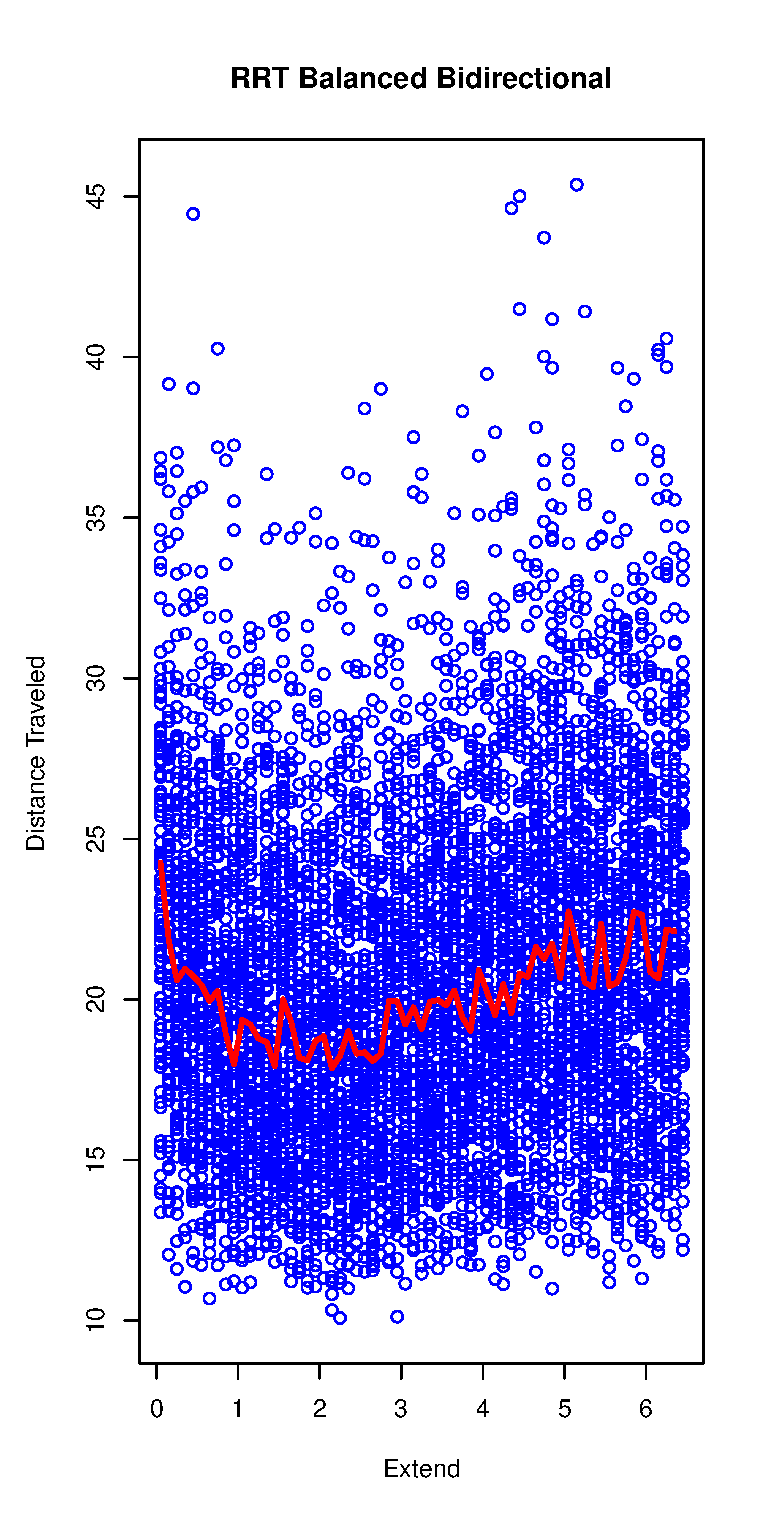
\includegraphics[width=\figsize]{graphics/balanced_correlation}
 \caption{\(d_J\) of the balanced bidirectional RRT planner (blue) with median highlighted (red).}
 \label{fig:balanced_correlated}
\end{figure}

% comparative

\begin{figure}[h]
 \centering
 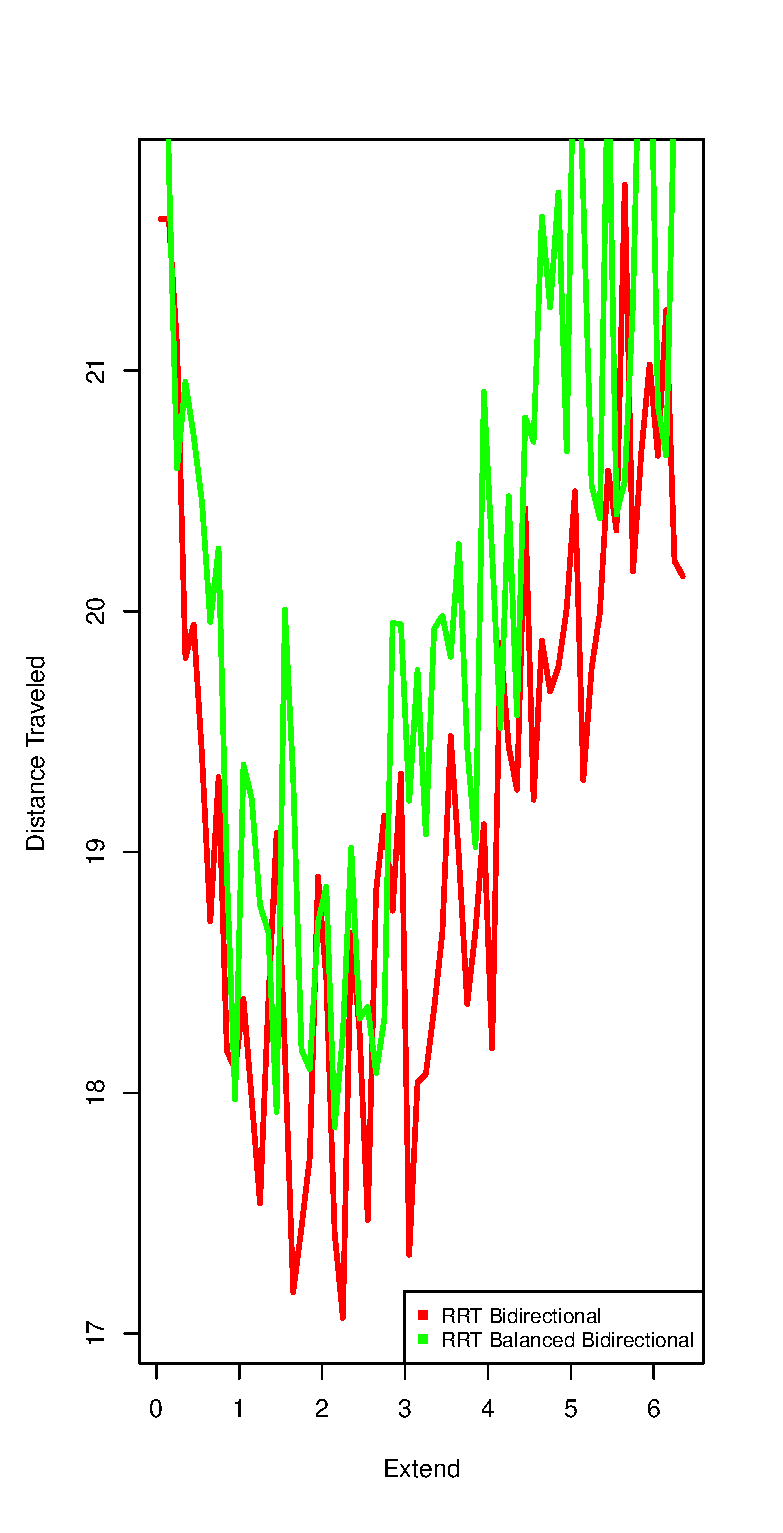
\includegraphics[width=\figsize]{graphics/compare_distance}
 \caption{Medians of \(d_J\) for the RRT planners.}
 \label{fig:medians}
\end{figure}

\begin{figure}[h]
 \centering
 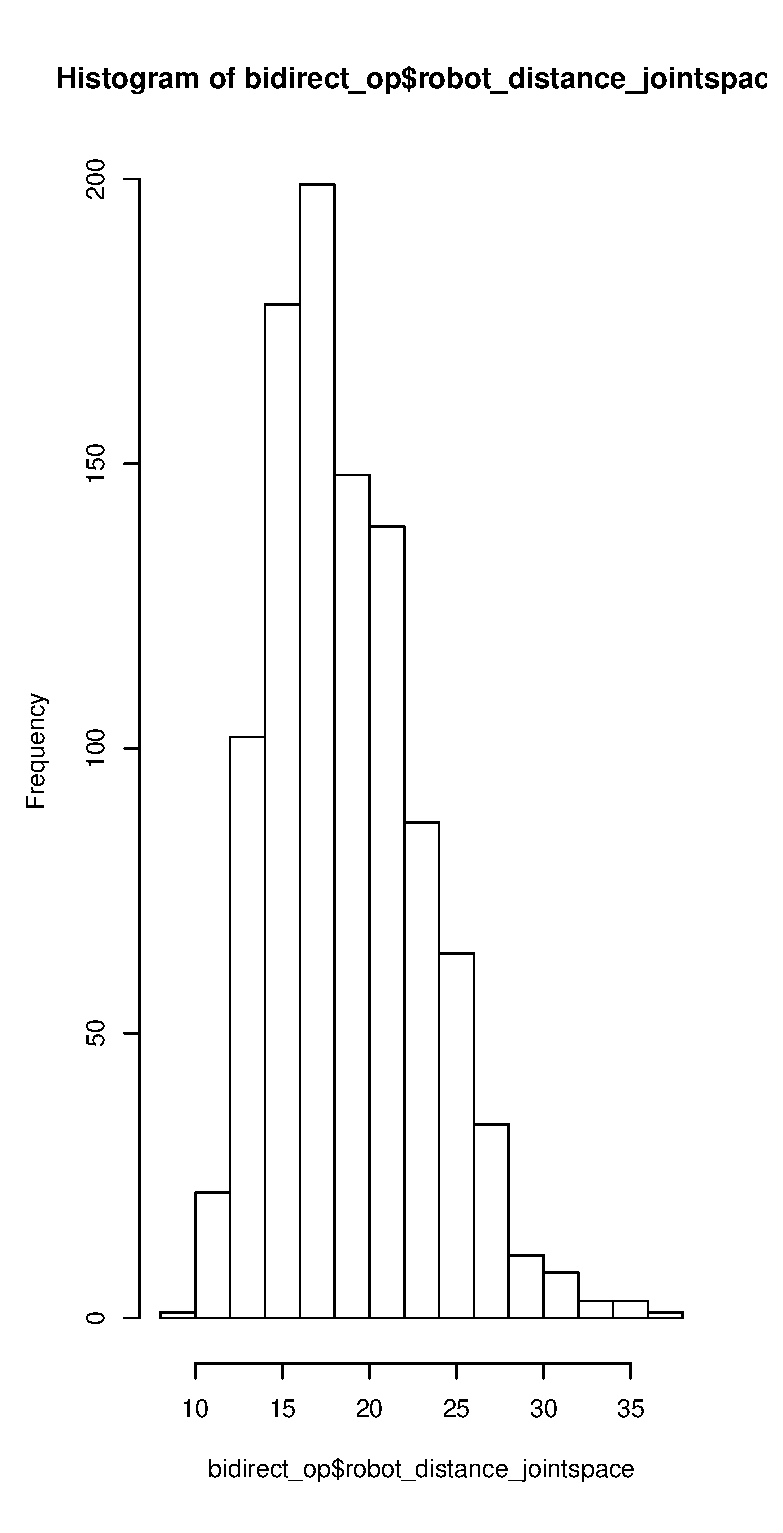
\includegraphics[width=\figsize]{graphics/hist_op_bi}
 \caption{Histogram for \(d_J\) with the optimal \(\epsilon\) for the bidirectional RRT planner.}
 \label{fig:bidir_histogram}
\end{figure}

\begin{figure}[h]
 \centering
 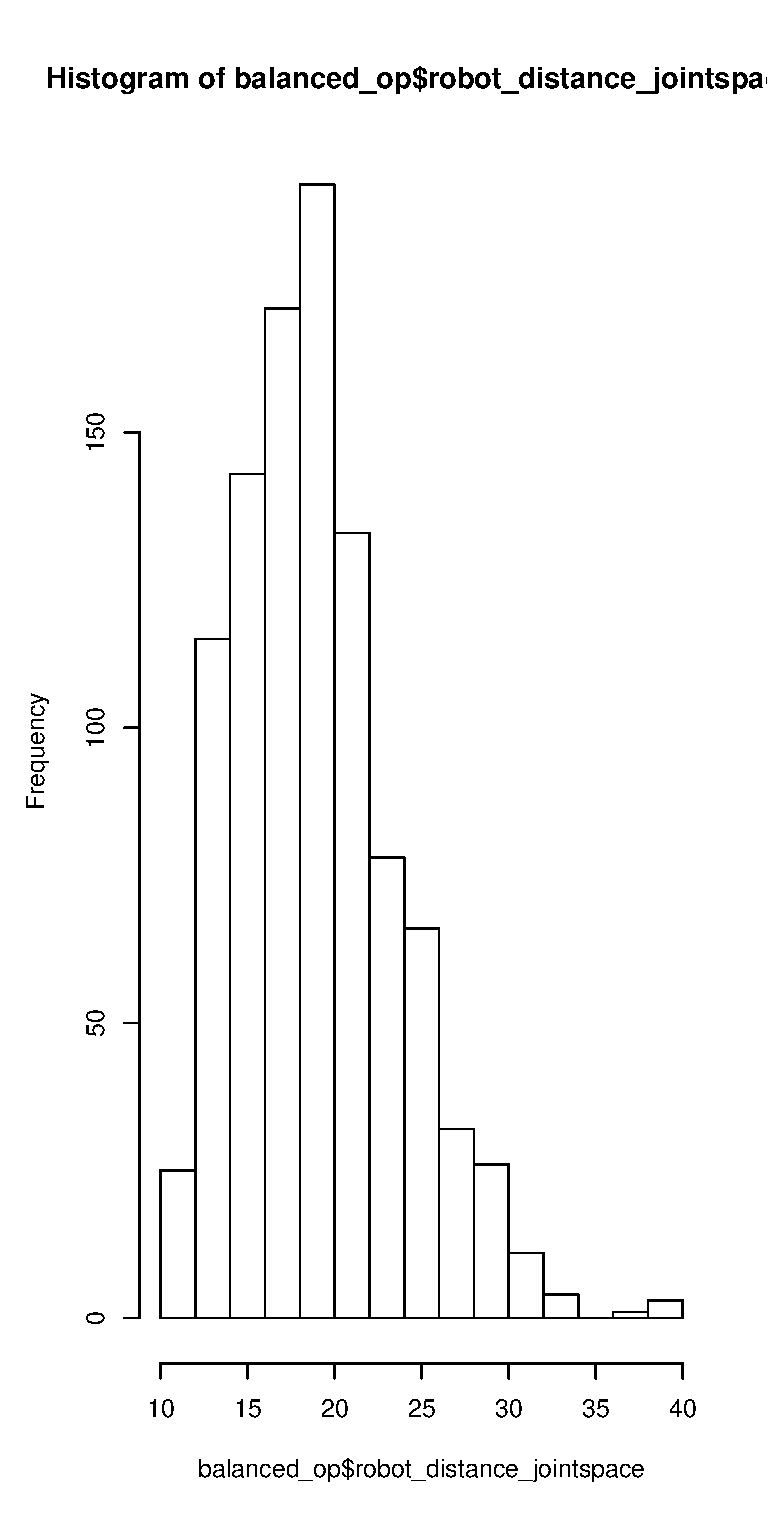
\includegraphics[width=\figsize]{graphics/hist_op_ba}
 \caption{Histogram for \(d_J\) with the optimal \(\epsilon\) for the balanced bidirectional RRT planner.}
 \label{fig:balanced_histogram}
\end{figure}

\begin{figure}[h]
 \centering
 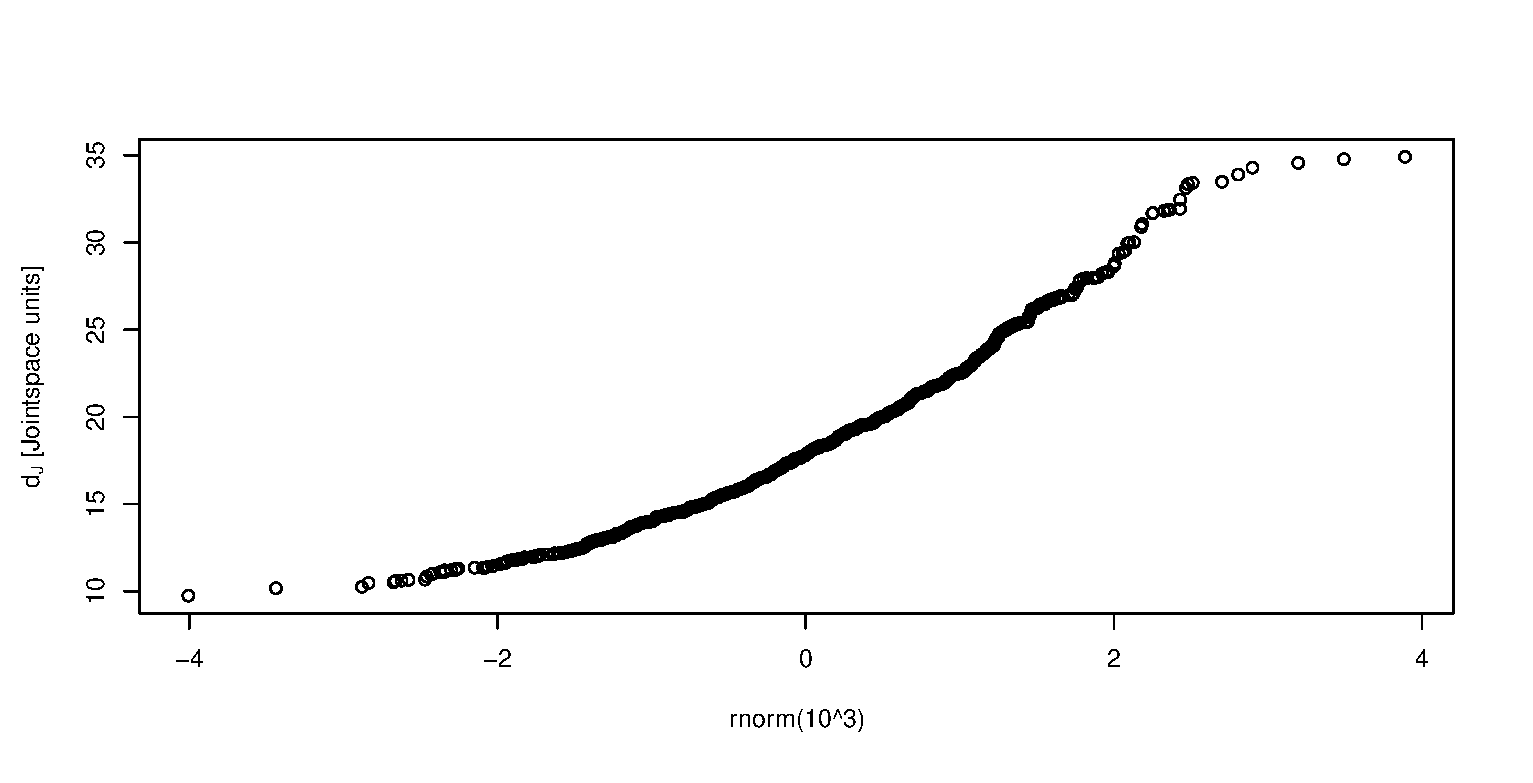
\includegraphics[width=\figsize]{graphics/qq_op_bi}
 \caption{Normal QQ plot for \(d_J\) with the optimal \(\epsilon\) for the bidirectional RRT planner. The normal distribution is approximated with 1000 samples.}
 \label{fig:bidir_qq}
\end{figure}

\begin{figure}[h]
 \centering
 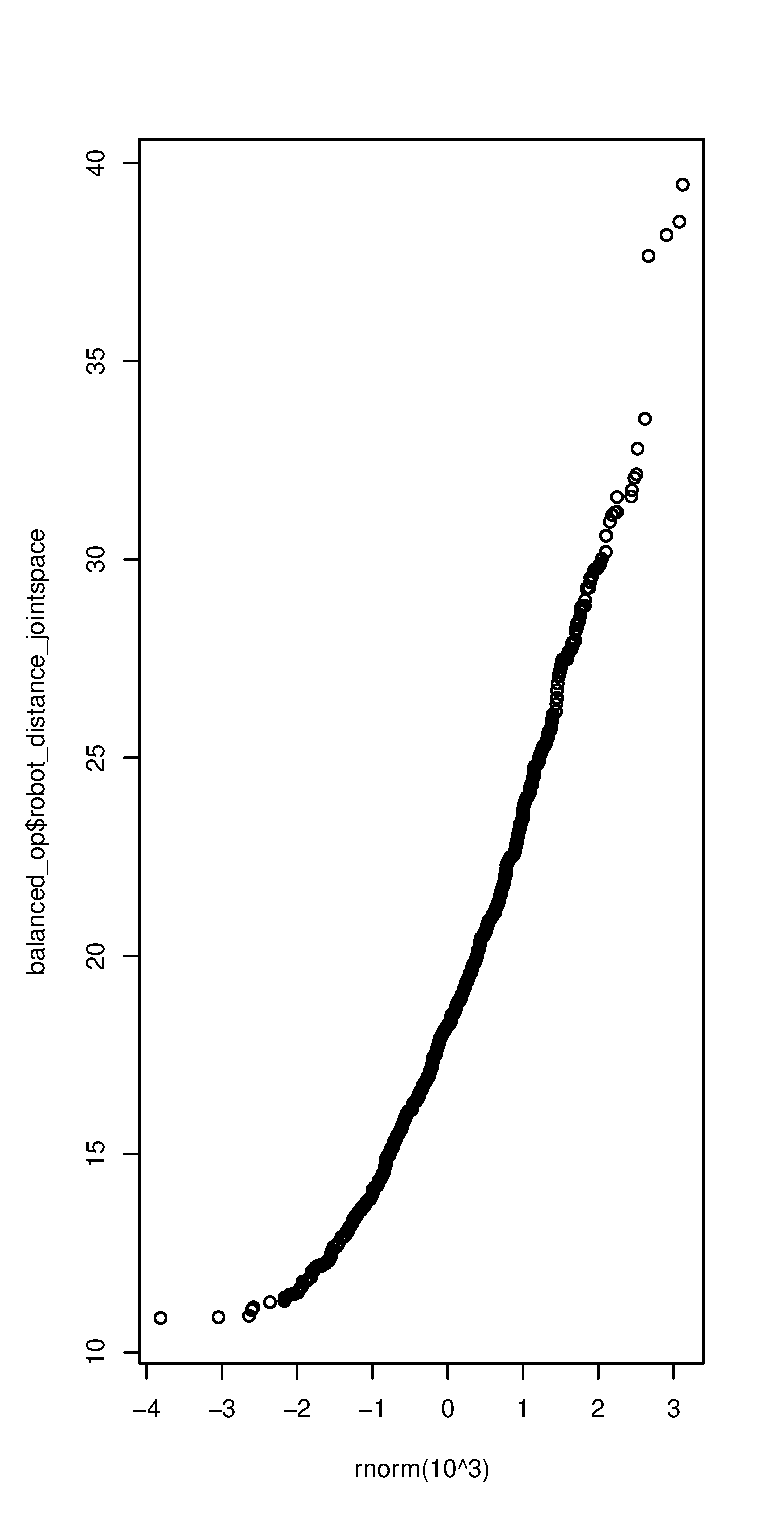
\includegraphics[width=\figsize]{graphics/qq_op_ba}
 \caption{Normal QQ plot for \(d_J\) with the optimal \(\epsilon\) for the balanced bidirectional RRT planner. The normal distribution is approximated with 1000 samples.}
 \label{fig:balanced_qq}
\end{figure}

\begin{figure}[h]
 \centering
 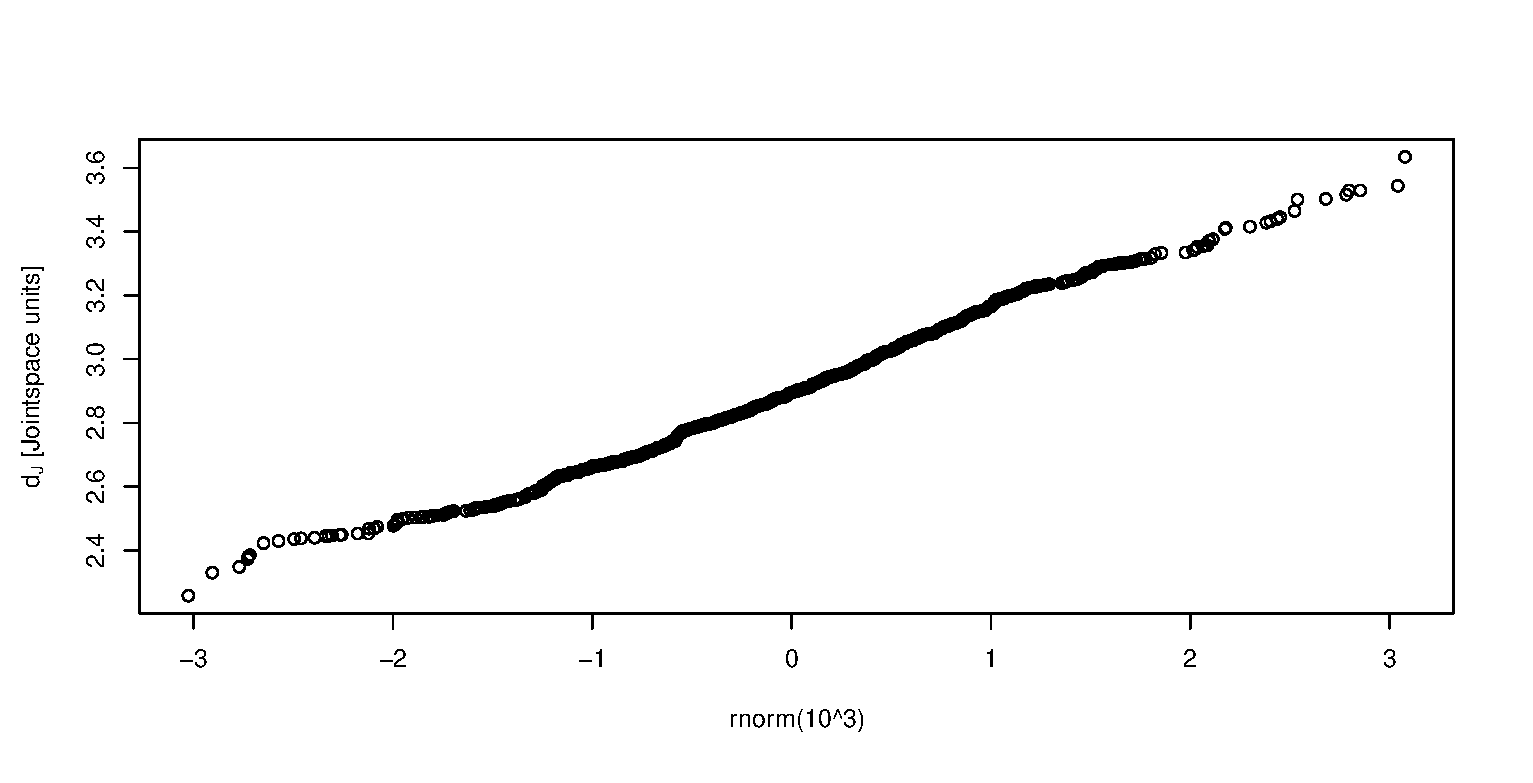
\includegraphics[width=\figsize]{graphics/qq_tran_op_bi}
 \caption{Normal QQ plot for the log transformed \(d_J\) with the optimal \(\epsilon\) for the bidirectional RRT planner. The normal distribution is approximated with 1000 samples.}
 \label{fig:bidir_log_qq}
\end{figure}

\begin{figure}[h]
 \centering
 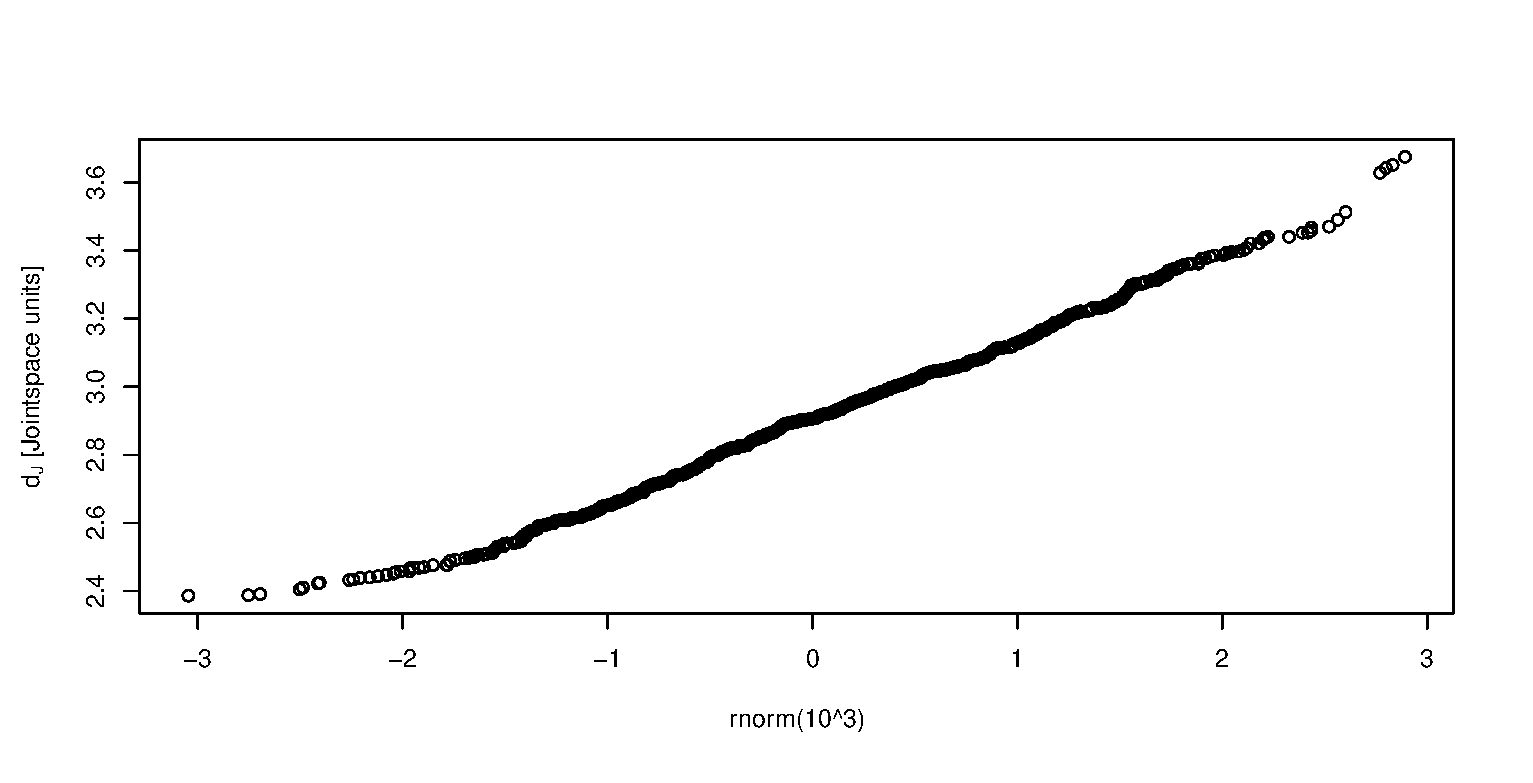
\includegraphics[width=\figsize]{graphics/qq_tran_op_ba}
 \caption{Normal QQ plot for the log transformed \(d_J\) with the optimal \(\epsilon\) for the balanced bidirectional RRT planner. The normal distribution is approximated with 1000 samples.}
 \label{fig:balanced_log_qq}
\end{figure}



